\documentclass[12pt,a4paper]{article}
\usepackage[latin1]{inputenc}
\usepackage{amsmath}
\usepackage{amsfonts}
\usepackage{amssymb}
\usepackage{graphicx}



\begin{document}
\begin{titlepage}
   \begin{center}
       \vspace*{1cm}
 
       \textbf{{\huge Verslag Roadfighter}}
 
       \vspace{0.5cm}
        Project gevorderd programmeren
 
       \vspace{1.5cm}
 
       \textbf{{\Large Stijn Rosaer}\\20172195}
  
       \vspace{10cm}
 
       
\includegraphics[scale=0.4]{img/logoua.jpg}

       Januari 2019
 
   \end{center}
\end{titlepage}
\newpage

\section{Idea}
Het idee is om een spel te cre\"eren waarbij men zo goed mogelijk de finish moet bereiken met een zo hoog mogelijk puntensaldo. Dit kan door auto's neer te schieten, speciale auto's aan te rijden en te proberen andere voertuigen te vermijdenn.

\section{Game}
Het spel werkt vanuit een klasse Game die alles zal controleren en in een juiste volgorde zal oproepen. Deze vormt dus de centrale plaats om controles uit te voeren op de status van het spel, waardoor ik besloten heb om hier de parameters (distance, score, background, factory, world, \ldots) bij te houden.\\
De World bezit alle objecten die tijdens het spel voorkomen. Deze komen daar terecht door middel van abstract factoring en worden terug gegeven als shared entity pointers. Wanneer een object verwijderd moet worden, zal dit ook van hieruit gebeuren.\\
Een update van alle elementen gebeurt eveneens vanuit World. Door composition design patern zal ik van hieruit voor elke bijgehouden entity de update aanroepen. Draw zal op dezelfde manier uitgevoerd worden.\\
\linebreak
Om het spel "speelbaar" te maken en een constante snelheid te hebben op verschillende computers start in het begin van elke loop over mijn spel een timer/ Op het einde wacht ik dan de resterende tijd nodig om een frame rate te bekomen van 30 fps.\\
Het genereren van een passing car, is afhankelijk van een uitgevoerde wiskundige berekening die een hogere waarde zal terug geven in fuctie van je snelheid en progressie in het spel. Op deze manier wordt een evenwicht aan auto's op de weg bekomen. Elke keer dat een passing car aangemaakt wordt zal deze met 10\% kans een special passing car zijn\\
\linebreak
Door het gebruik van observer patern kan ik doorgeven vanuit mijn observables (PlayerCar, Bullet en PassingPointsCar) welke actie er in de overeenkomstige observer (Game) uitgevoerdt moet worden.
\newpage

\section{Objects}
Elk object bezit de nodige parameters op de meest voor de hand liggende plaats in de minst afgeleide klasse. Zo bevind zich de struct boundries zich in entity welke een top left, botom right, center, width en height bevat waardoor deze gemakkelijk door gegeven kunnen worden.\\
Voor het controleren van collisions heb ik er voor gekozen om deze functie te implementeren in Entity. Dit leek me logisch omdat een entity botst met anderen. Hiervoor geef ik een vector mee van entities waardoor ik dan zelf kan kiezen welke botsingen effectief een gevolg hebben.\\
Elk object wordt volledig vanuit de logische kant gecontroleerd. Dit betekenet dat beslissingen en bewegingen van hieruit gestuurd worden en dat de graphische kant enkel voor het displayen is. In de grafische module zal dus ook de transformation singleton gebruikt worden om de omzetting van logische co\"ordinaten naar pixel co\"ordinaten te doen.

\section{Background \& movement}
Om een perceptie van snelheid te cre\"eren heb ik de achtergrond als een lus door laten lopen aan de snelheid van de speler. Elk ander object krijgt een eigen snelheid. In de update functie zal de snelheid van de speler mee door gegeven worden. Hieruit kan de relatieve snelheid worden berekend en de relatieve verplaatsing van het object.

\section{Racing car \& special passing car}
\subsection{Racing car}
Voor de racing car heb ik gekozen om een simpele autonomie te implementeren. Dit heb ik verkregen door elke keer dat de auto een object raakt, er een 90\% kans is dat hij dit object zal ontwijken met een gelijke verdeling links en rechts. Deze hitrate komt overeen met een normaal persoon.\\
Doordat de racing car geen rekening houdt met de speler, heb ik de keuze genomen dat deze eigenlijk dezelfde race rijd als de speler, maar zonder interactie tussen beiden. We kunnen dus eigenlijk zeggen dat de racing car een ghost player is. 

\subsection{Special passing car}
Als tweede soort passing car heb ik beslist om een auto te maken die, wanneer geraakt wordt, zorgt voor extra punten. Voor de rest heeft deze exact dezelfde eigenschappen als een normale passing car.

\section{Interaction}
Hieronder is een overzicht te vinden van de inheritance tussen de voornaamste klassen. Extra schemas en documentatie zijn te vinden in de DOC folder gegenereerd door doxygen.\\
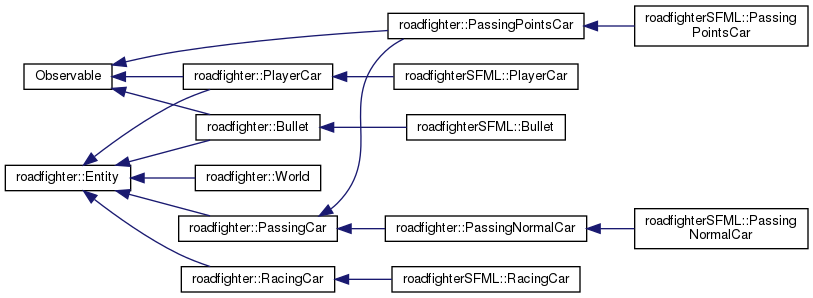
\includegraphics[scale=0.5]{img/inherit_graph_2.png}
\end{document}